\subsection{Ist-Analyse}
\label{sec:IstAnalyse}

Momentan lassen sich Informationen über die angebotenen Studiengänge am Studien-
standort Lingen über die Hochschulseite \url{www.hs-osnabrueck.de} abrufen. Diese Internetseite bietet dabei weiterführende
Links mit Informationen für Studierende und Unternehmen. Hier werden zum Beispiel Labore, Projekte und Dozenten der
Hochschule vorgestellt. Darüber hinaus werden in einer Bildergalerie einzelne Impressionen des neuen Campus dargestellt.
Ein Bildschirmfoto dieser Internetseite ist in \abbildung{Bildergalerie} abgebildet.

\clearpage

\begin{figure}[htb]
\centering
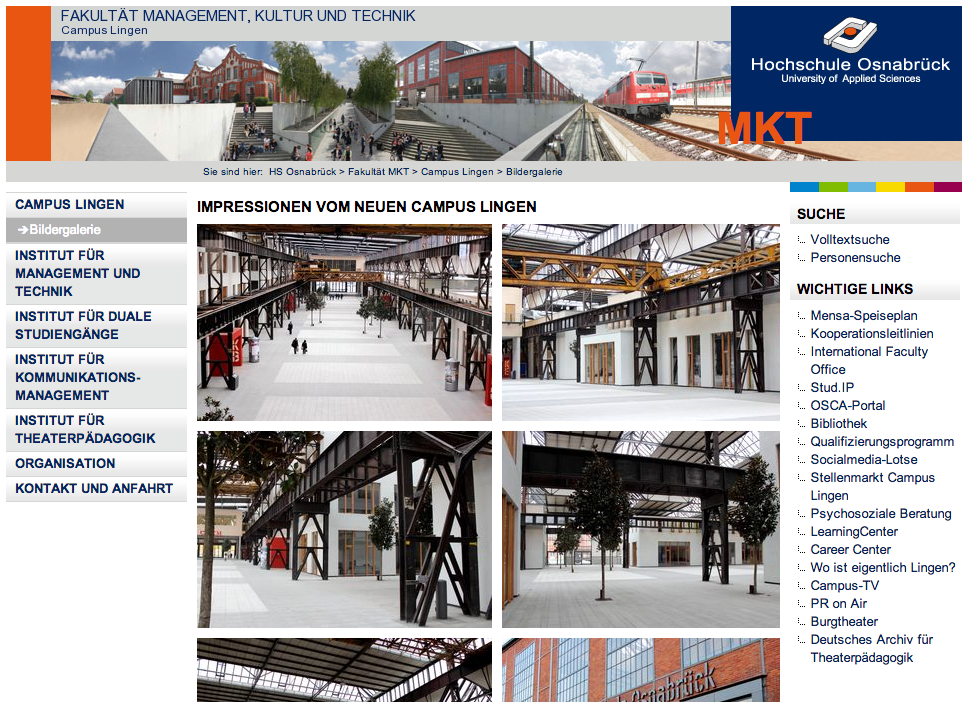
\includegraphics[width=1.0\textwidth]{Bildergalerie.png}
\caption[Bildergalerie des Campus Lingen]{Bildergaliere des Campus Lingen\protect\footnotemark}
\label{fig:Bildergalerie}
\end{figure}
\footnotetext{Link: http://www.campus-lingen.hs-osnabrueck.de}

Ähnlich wie die Informationsvermittlung auf der Internetseite der Hochschule Osnabrück
gestaltet sich auch die Informationsvermittlung auf Messen. Diese Messen bieten Studieninteressierten die Möglichkeit
sich über die einzelnen Studienangebote erkundigen können. Dort werden ebenfalls
Impressionen des Campus in Lingen gezeigt oder Informationsmaterial verteilt.

Im Zuge dieser Analyse wurden zwei Elemente heraugestellt, welche vor dem Hintergrund der Projektidee wiederverwendet
werden können.

\textbf{1.} Die Fotos, die bereits vom neuen Campus gemacht wurden.

\textbf{2.} Das Informationsmaterial das über Projekte, Studiengänge, Dozenten und weiteres zusammen getragen wurde.

Die bereits angefertigen Fotos können dabei nicht für das vorliegende Projekt verwendet werden, da es sich bei diesen 
Fotos nicht um 360-Grad-Fotos handelt. Darüber hinaus sind auf diesen Fotos nur einzelne Impressionen des Campus 
dargestellt und keine umfassenden Einblicke. Die bestehenden Impressionen zeigen aber
interessante Blickwickel des Campus. Diese Blickwinkel können bei der Erstellung der neuen Fotos aufgegriffen werden. 


Das auf der Internetseite der Hoschule zusammengetragene Informationsmaterial kann kann dagegen verwendet werden, um 
Informationen zu bestimmten Panoramas anzuzeigen. Für die Rechereche nach Informationsmaterial kann daher Aufwand im Projekt eingespart werden.